%%%% fs-run-time-experiments   Experiments

\label{fs-experiments-section}

We evaluated the prototype of the system by incrementally computing inverted index.

The computation of inverted index is implemented in terms of MapReduce transformations. We start with page mapping into the pairs {\it (word; word positions within the page)}. After that, word positions are reduced by word into the single structure. We assume the output of the stream to be a change log of the inverted index structure. More precisely, each input page should trigger the output of the corresponding changelog. 

In the real-world, such scenario can be found in freshness-aware systems e.g. news processing engines. By the notion of {\it latency} we assume the time between two events: 
\begin{enumerate}
    \item Input page is taken into the stream;
    \item The last item of the corresponding changelog leaves the stream.
\end{enumerate}

In \FlameStream\ this algorithm is implemented as the typical conversion of MapReduce transformation, which is shown in the section~\ref{fs-map-reduce}. Inverted index structure plays the role of accumulator, and the accumulator map produces the most recent changes of this structure, if any.

The same task was executed by Apache Flink for performance comparison. For Apache Flink, this algorithm is adopted by the usage of {\it FlatMapFunction} for map step and stateful {\it RichMapFunction} for reduce step and for producing the changelog.

Our experiments were performed on clusters of 1,2,5,7, and 10 nodes. Each node is an Amazon EC2 micro instance with 1GB RAM and 1 core CPU. We used 10000 Wikipedia articles as a dataset. 

The latencies of \FlameStream\ across multiple workers are shown on the figures~\ref{fs-index-median} and~\ref{fs-index-quantiles}. These figures demonstrate the scalability of the system in terms of latency.

\begin{figure}[htbp]
  \centering
  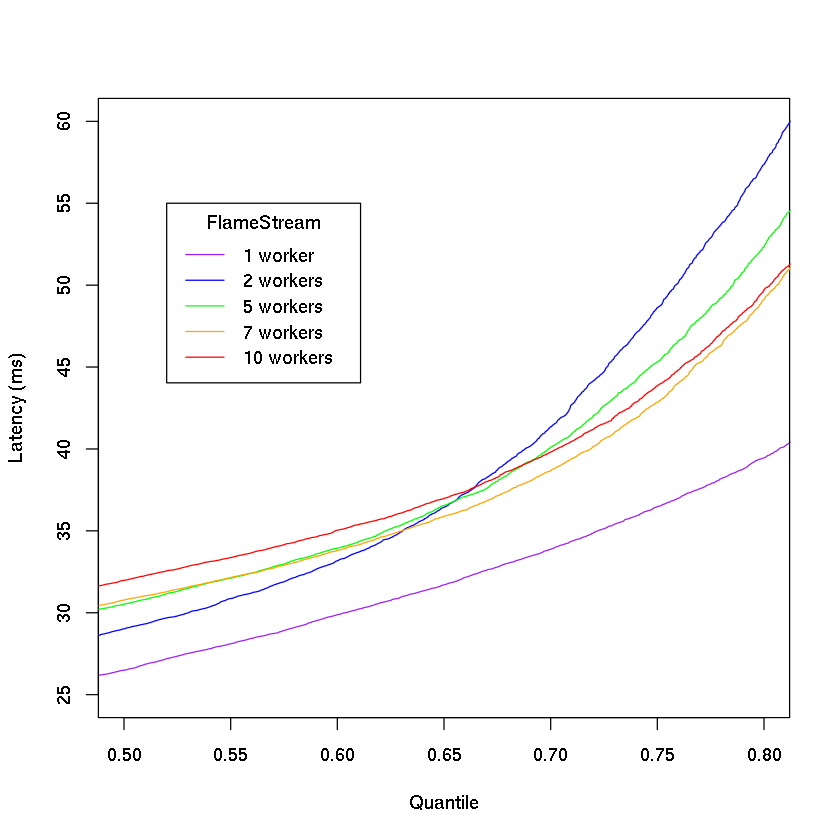
\includegraphics[width=0.48\textwidth]{pics/fs-index-median}
  \caption{FlameStream median latencies}
  \label {fs-index-median}
\end{figure}

\begin{figure}[htbp]
  \centering
  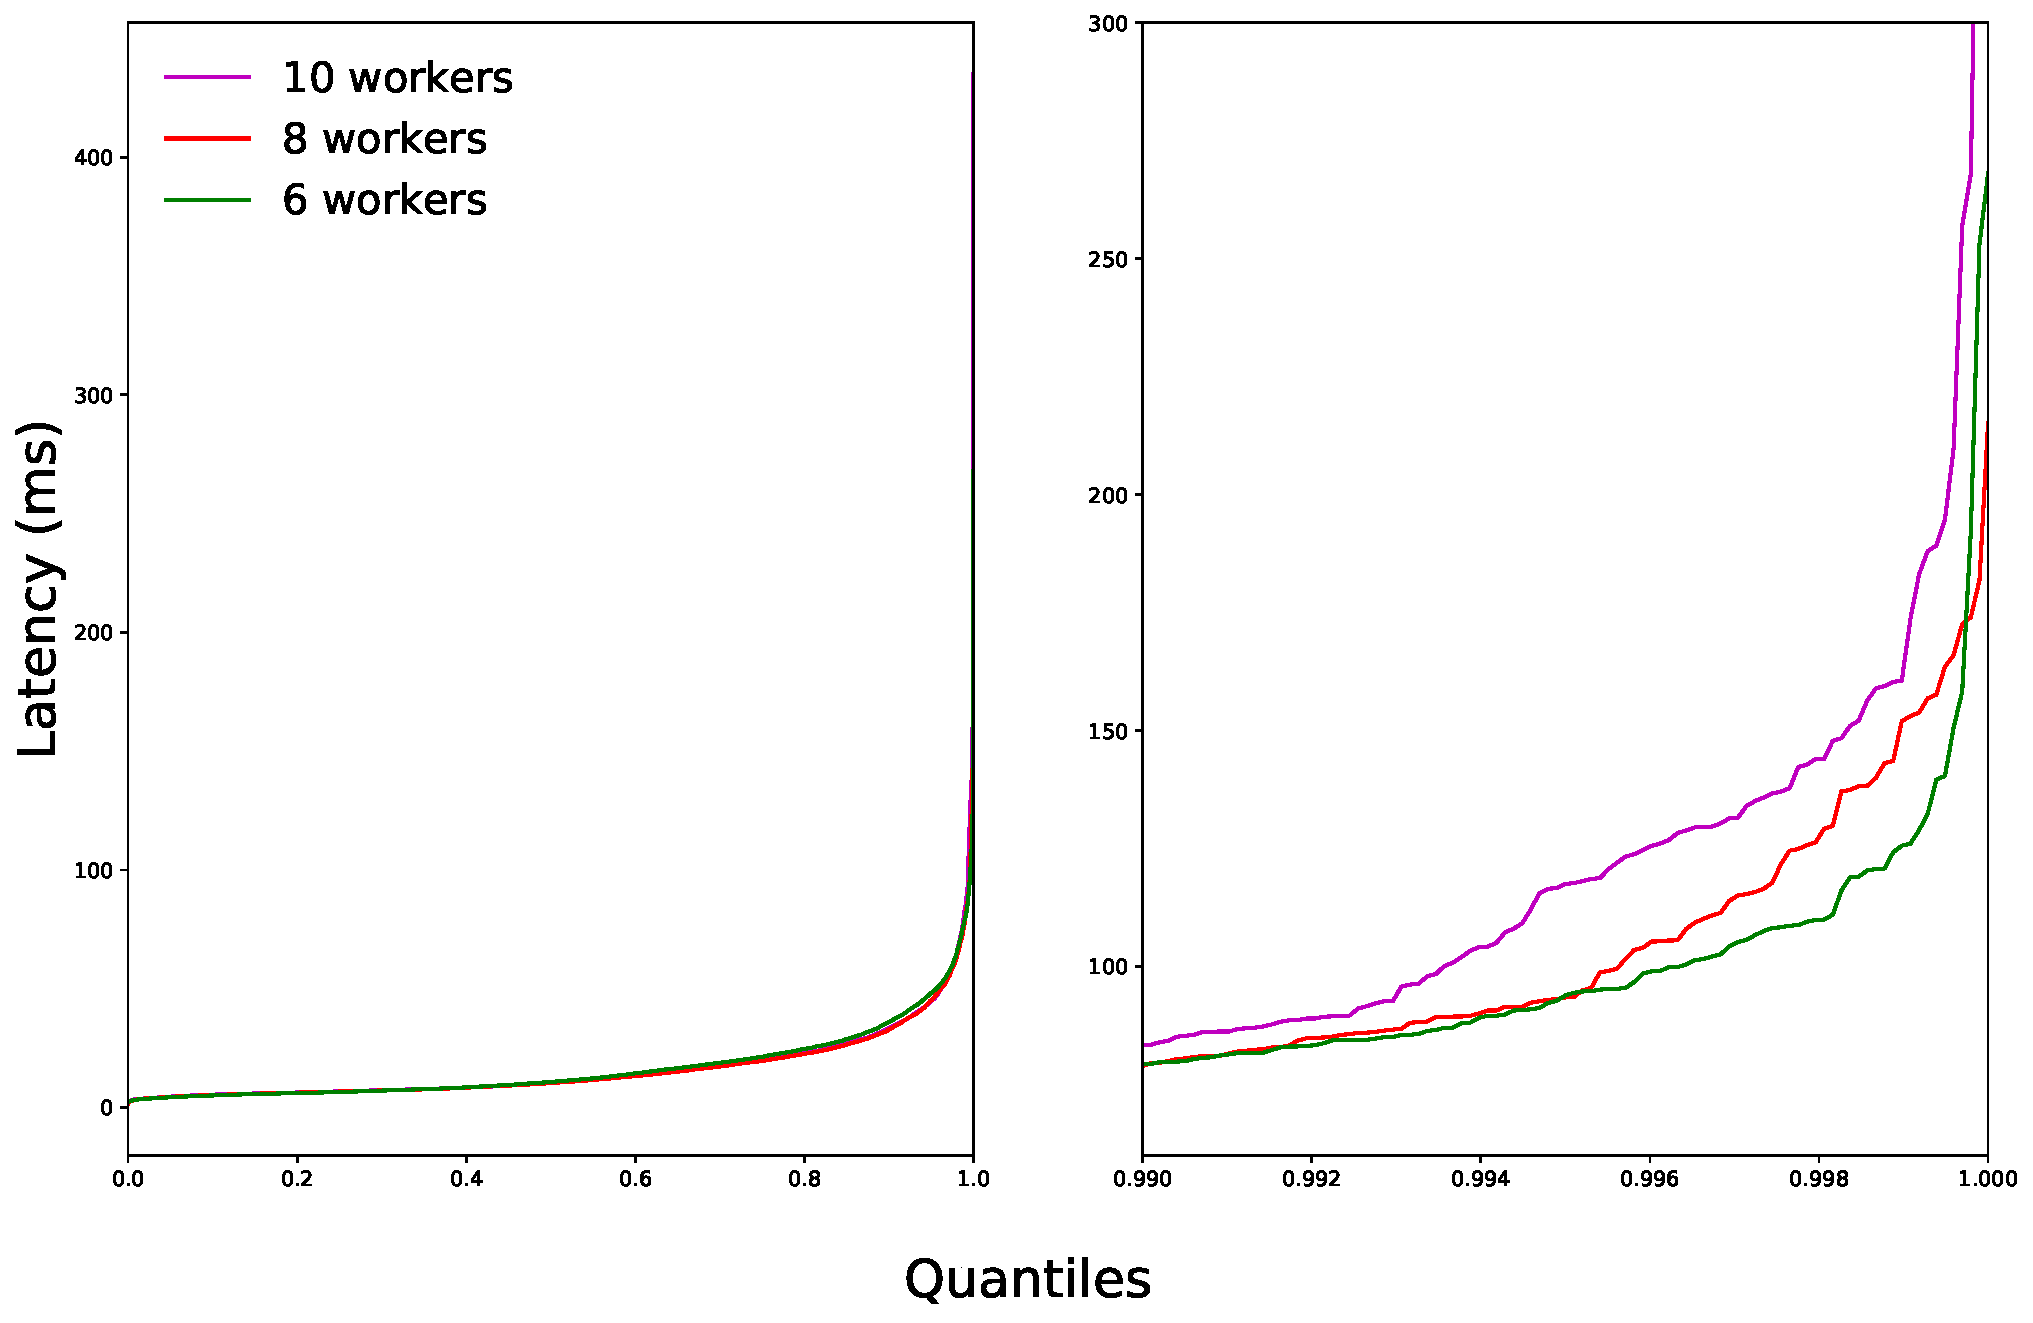
\includegraphics[width=0.48\textwidth]{pics/fs-index-quantiles}
  \caption{FlameStream tail latencies}
  \label {fs-index-quantiles}
\end{figure}

The comparison in latencies between FlameStream and Flink within 10 nodes is shown on the figure~\ref{comp-index-quantiles}. These results show that \FlameStream\ is able to deliver better latency.

\begin{figure}[htbp]
  \centering
  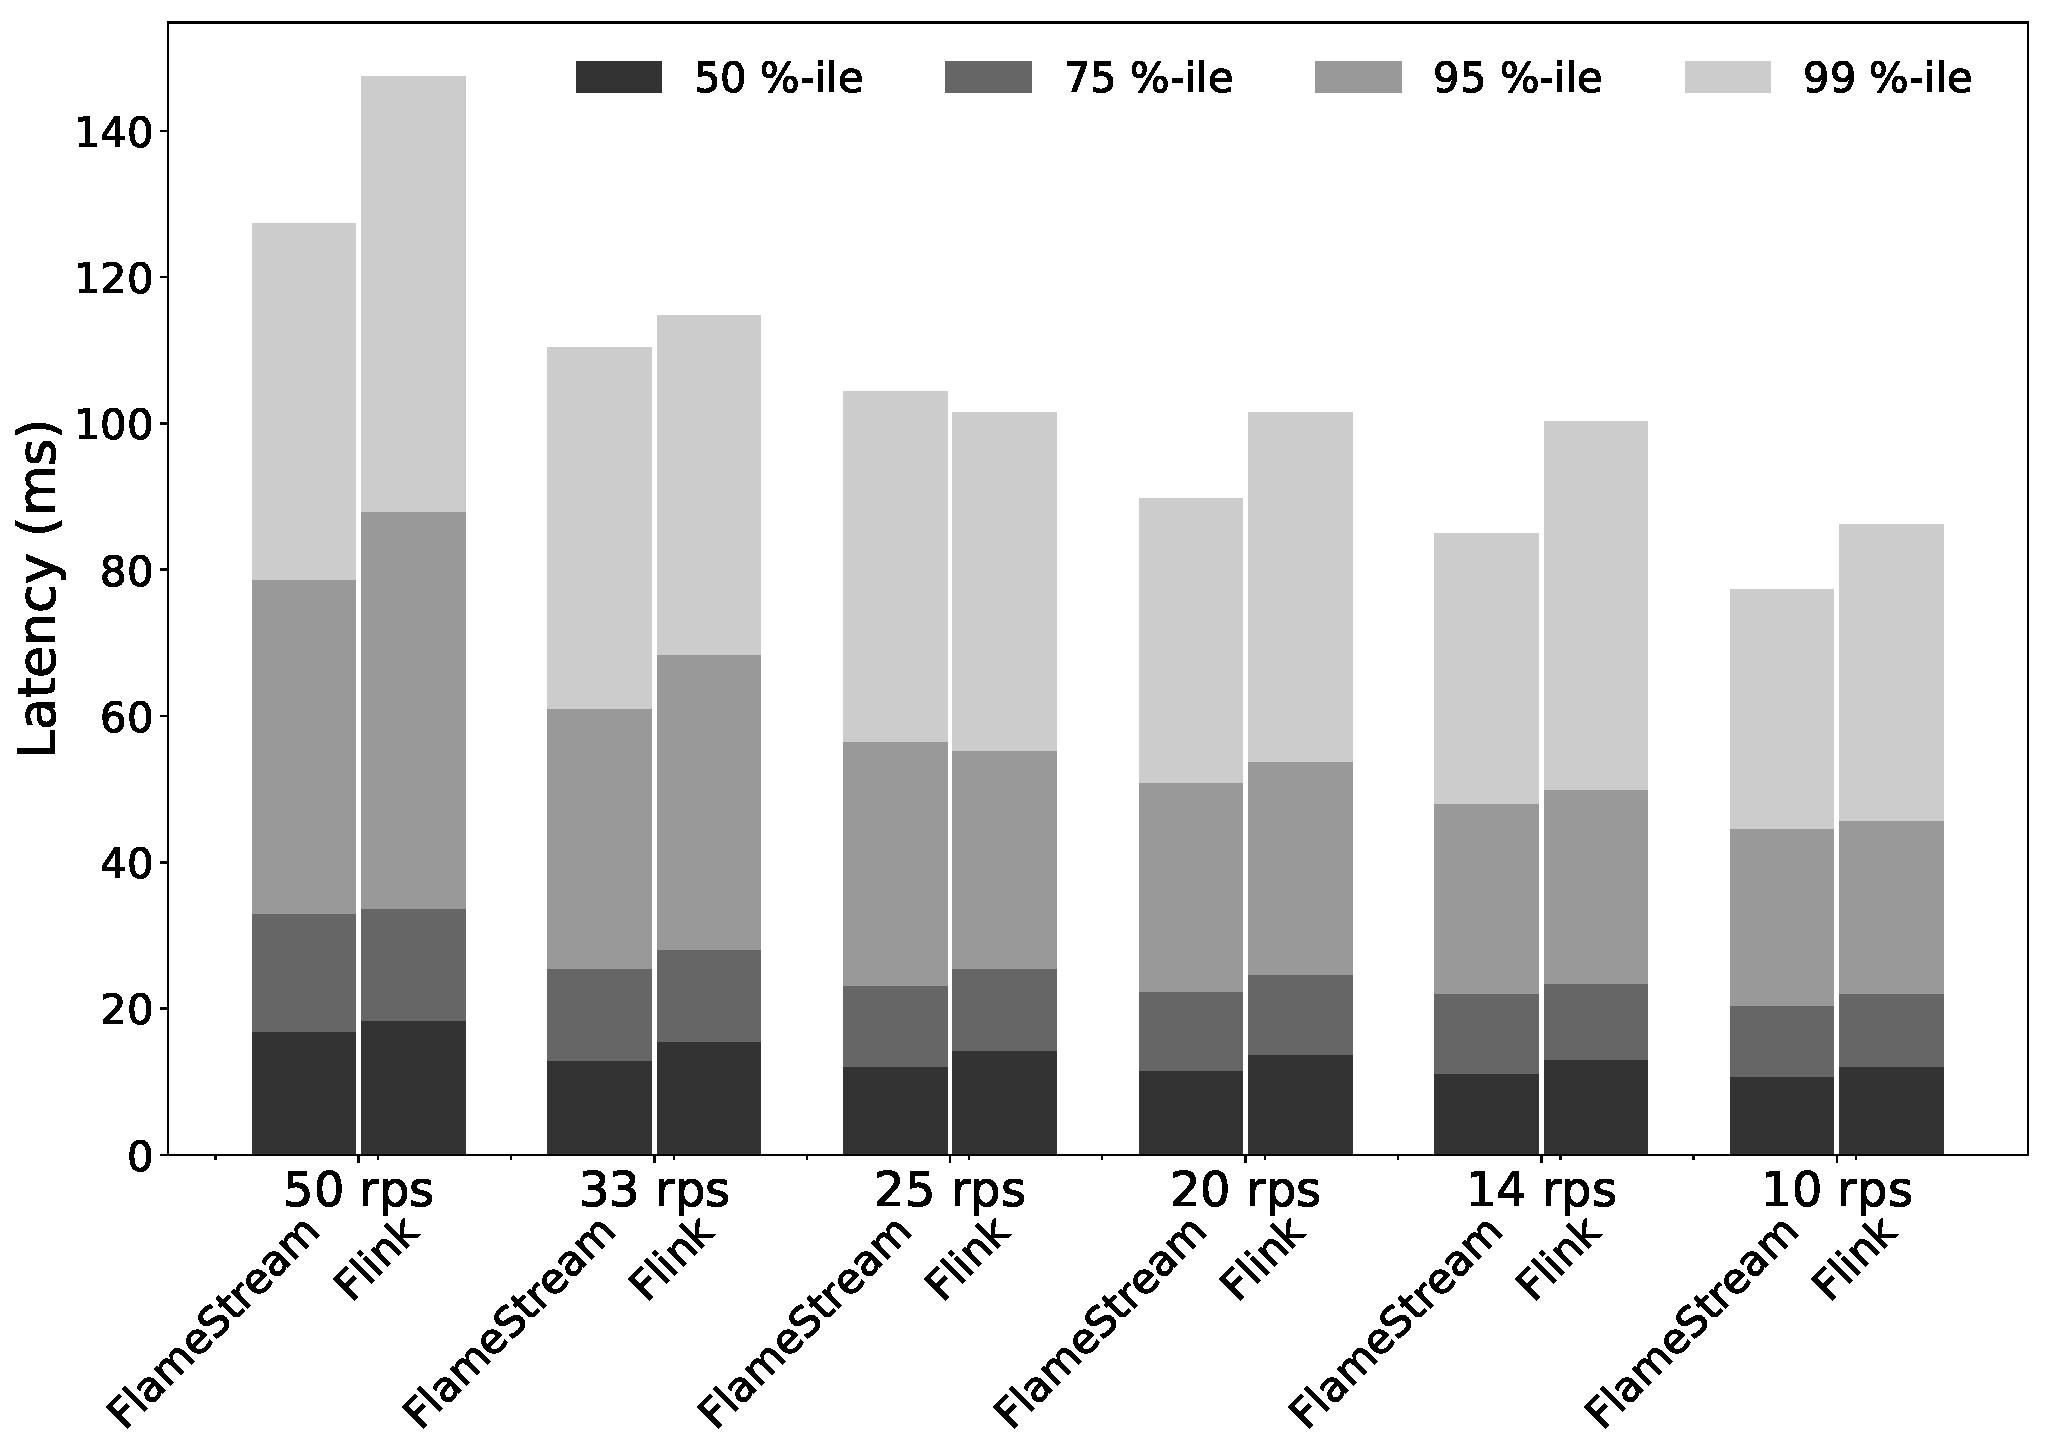
\includegraphics[width=0.48\textwidth]{pics/comp-index-quantiles}
  \caption{Apache Flink and FlameSream latency distribution comparison}
  \label {comp-index-quantiles}
\end{figure}
